\documentclass[11pt]{article}
\usepackage{listings}
\usepackage{xcolor}
\usepackage{graphicx}
\usepackage{float}

\definecolor{codegreen}{rgb}{0,0.6,0}
\definecolor{codegray}{rgb}{0.5,0.5,0.5}
\definecolor{codepurple}{rgb}{0.58,0,0.82}
\definecolor{backcolour}{rgb}{0.95,0.95,0.92}

\lstdefinestyle{mystyle}{
    backgroundcolor=\color{backcolour},   
    commentstyle=\color{codegreen},
    keywordstyle=\color{magenta},
    numberstyle=\tiny\color{codegray},
    stringstyle=\color{codepurple},
    basicstyle=\ttfamily\footnotesize,
    breakatwhitespace=false,         
    breaklines=true,                 
    captionpos=b,                    
    keepspaces=true,                 
    numbers=left,                    
    numbersep=5pt,                  
    showspaces=false,                
    showstringspaces=false,
    showtabs=false,                  
    tabsize=2
}

\lstset{style=mystyle}

\begin{document}
\title{Matematica in Latex}
\author{Calabrigo Massimo}
\date{\today}
\maketitle

\tableofcontents
\section{Introduzione}
Il nostro obiettivo è creare un database postgres, per la gestione di uno studio medico.
Vogliamo registrare informazioni sulle sedute e le terapie dei pazienti, sulle competenze e gli orari di lavoro dei medici, e degli altri dipendenti.
\section{Requisiti e Specifiche}

\subsection{Workflow e fase di specificazione}
Per questo progetto abbiamo deciso di utilizzare un modello iterativo incrementale.
Abbiamo separato il progetto in tre processi: Requisiti e specifiche, Progettazione ed Implementazione;
a loro volta divisi in sottoprocessi:
\begin{enumerate}
    \item Requisiti e Specifiche
    \begin{itemize}
        \item Analisi: lettura del documento, evidenziando punti importanti
        \item Specificazione: riassumere i punti importanti nelle specifiche
        \item Validazione: controllo che le specifiche rispettino il documento, eventualmente tornando all'analisi
    \end{itemize}
    \item Progettazione
    \begin{itemize}
        \item concettuale: stesura e ristrutturazione dell'ER dalle specifiche
        \item logica: traduzione da ER a logico, validazione, ed implementazione su postgres
        \item fisica: scelta degli indici
    \end{itemize}
    \item Implementazione
    \begin{itemize}
        \item Implementazione di operazioni e viste
        \item Analisi statistica dei dati
    \end{itemize}
\end{enumerate}
In questa sezione esponiamo il processo di "Requisiti e specifiche", e riportiamo
solo i risultati i risultati finali.

Come prima cosa abbiamo letto il documento con le richieste del cliente (fornito dal professore)
evidenziando concetti principali, annotandoli nel glossario, e richieste importanti. Poi abbiamo iniziato la prima fase di 
analisi dei requisiti, elencando e riordinando quello che avevamo evidenziato.
Prima di passare alla fase di specificazione abbiamo riletto requisiti e documento delle richieste cercando
incompletezze ed errori, quindi abbiamo raffinato i requisiti (seconda iterazione di requisiti).
Quindi siamo passati ad una prima iterazione delle specifiche, in cui abbiamo cominciato a
risolvere le ambiguità, documentando la soluzione nel glossario e semplificando la descrizione.
In una prima fase di validazione abbiamo notato che non erano chiari alcuni dettagli riguardanti
terapie prolungate ed appuntamenti, e se gli appuntamenti fossero da considerarsi sedute programmate;
Quindi siamo tornati all'analisi dei requisiti, risolvendo questo dubbio, ed abbiamo proseguito
con l'ultima fase di specificazione e validazione.

\begin{figure}[H]
    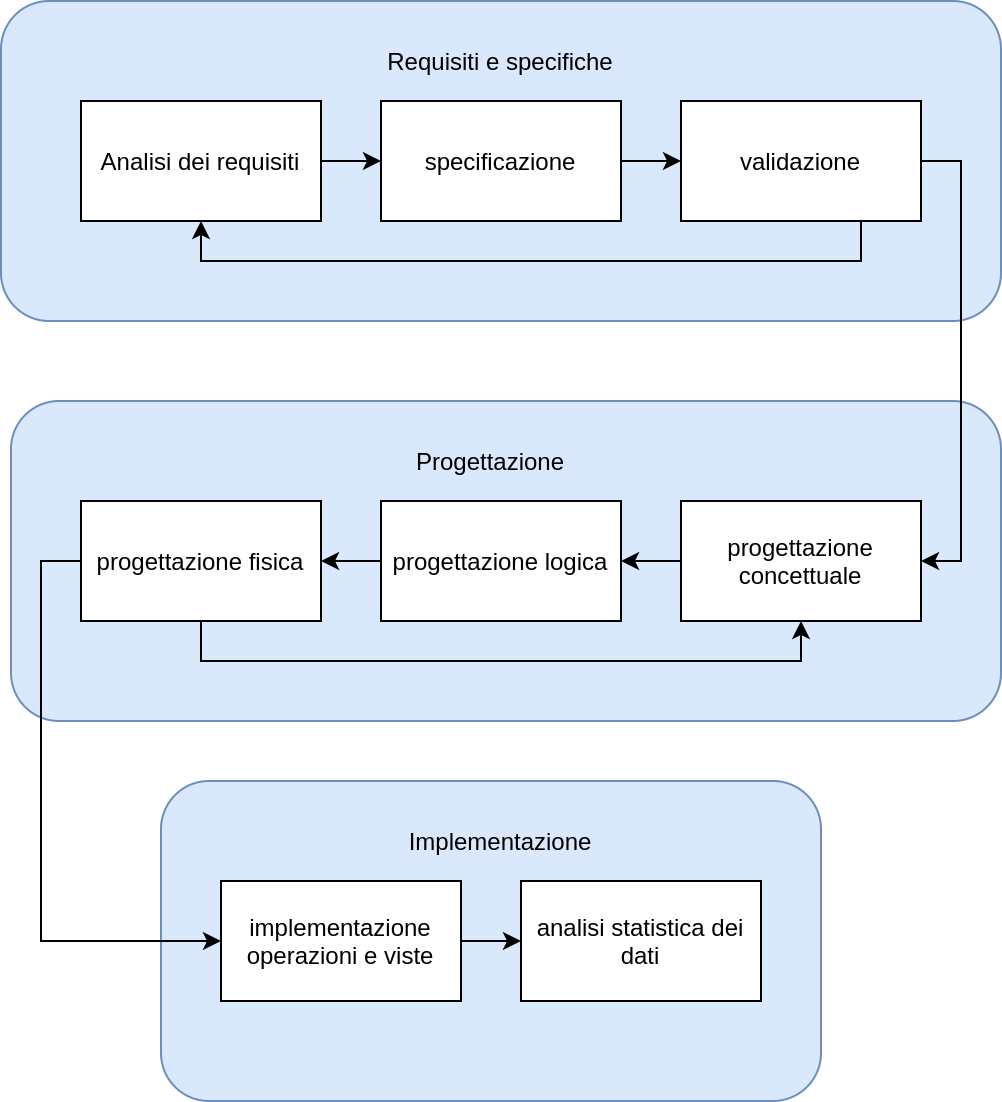
\includegraphics[width=\linewidth]{images/workflow.png}
    \caption{workflow}
    \label{fig:workflow}
\end{figure}
\subsection{Glossario}
Nel corso del processo di specificazione abbiamo annotato i vari termini specifici del
dominio, risolvendo le ambiguità. L'elenco riportato è riferito all'ultima iterazione di
requisiti e specifiche.
\begin{itemize}
\item Medico: Ogni medico può essere interno od esterno.
\item Medico interno: Medico comproprietario dello studio medico.
\item Medico esterno: Medico non comproprietario dello studio medico.
\item Codice-medico: Codice che identifica univocamente un medico.
\item Membro del personale ausiliario: Ogni membro può essere assistente medico, oppure amministrativo, può anche essere entrambe le cose.
\item Codice-personale: Codice che identifica univocamente un membro del personale ausiliario.
\item Paziente: cliente dello studio medico.
\item Paziente regolare: Paziente che si sottopone ad almeno una terapia prolungata.
\item Paziente occasionale: Paziente che si sottopone ad almeno una seduta per un problema urgente.
\item Specializzazione: Titolo di studio acquisito da tutti medici dopo la laurea. (Oculistica, urologia, cardiologia, …)
\item Qualifica: Titoli di studio specifici dei membri del personale ausiliario. (Diploma di ragioneria, laurea in infermieristica, tecnico radiologo, …)
\item Storico: Resoconto periodico.
\item Denominazione: Titolo di un corso di aggiornamento. (“Corso di aggiornamento in pneumologia”, …)
\item Terapia prolungata: Trattamento prolungato a cui si sottopone il paziente.
\item Seduta: Visita occasionale a cui si sottopone il paziente per motivi urgenti. La singola seduta deve risolvere il problema, altrimenti sarebbe parte di una terapia prolungata.
\item Appuntamento: Visita periodica a cui si sottopone il paziente come parte di una terapia prolungata. Quando ci si presenta ad un appuntamento viene comunicato un ambulatorio ed assegnati i membri del personale ausiliario ed i medici che si occuperanno della visita.
\item Appuntamento accettato: appuntamento a cui il paziente si presenta. Può essere terminato o ancora in corso.
\item Appuntamento saltato: appuntamento al quale il paziente non si è presentato.
\item Appuntamento programmato: appuntamento fissato per una data e ora future.
\end{itemize}
\subsection{Requisiti}
Abbiamo riportato requisiti finali, risultato dell'ultima (terza) iterazione di analisi dei requisiti.
Le iterazioni precedenti dei requisiti si trovano nel documento allegato "Specifiche.docx"
\begin{itemize}
    \item I \emph{medici} possono essere interni od esterni. Un medico è identificato univocamente da un codice-medico, ed ha un nome, un cognome, un indirizzo, un recapito telefonico, ed una o più \emph{specializzazioni}.
    \begin{itemize}
        \item I medici interni sono comproprietari ed hanno diritto su una percentuale degli incassi
        \item I medici esterni hanno una tariffa oraria
    \end{itemize}
    \item Ogni \emph{membro del personale ausiliario} è identificato univocamente da un codice-personale, ed ha un nome, cognome, indirizzo, recapito telefonico (uno), ed una o più qualifiche.
    \begin{itemize}
        \item Gli assistenti medici possono seguire dei corsi di aggiornamento.
        \item Amministrativi.
    \end{itemize}
    \item Ogni \emph{corso di aggiornamento} è identificato univocamente dalla denominazione, dal luogo dove si svolge, dalla data in cui si svolge. Due o più corsi di aggiornamento con la stessa denominazione non possono svolgersi nello stesso luogo alla stessa data.
    \item Ogni mese viene memorizzato \emph{uno storico delle ore lavorative} ordinarie e straordinarie dei medici e dei membri del personale ausiliario.
    \item I \emph{pazienti} possono essere regolari od occasionali. Un paziente è identificato univocamente dal codice fiscale, ed ha un nome, un cognome, un indirizzo, un recapito telefonico, ed una data di nascita.
    \begin{itemize}
        \item I pazienti occasionali si presentano allo studio per un problema urgente da risolvere in una seduta.
        \item I pazienti regolari si sottopongono ad una o più terapie prolungate. Un paziente regolare può essere anche occasionale per un problema urgente estraneo alla terapia prolungata.
    \end{itemize}
    \item Ogni \emph{seduta} è caratterizzata da le persone coinvolte (un paziente, uno o più medici, uno o più membri del personale ausiliario), dalla data, l’ora, e l’ambulatorio in cui si svolge la seduta.
    \item Ogni \emph{terapia prolungata} è caratterizzata dal paziente, da uno specifico tipo di medico e da una data di fine. Una terapia prolungata può essere aperta o chiusa, inizialmente è aperta e quando termina diventa chiusa. Ad un paziente in terapia prolungata aperta possono essere associati uno o più appuntamenti programmati, mentre ad una terapia prolungata chiusa solo appuntamenti accettati o saltati.
    \begin{itemize}
        \item Gli appuntamenti possono essere programmati. In seguito, se il paziente si presenta all’ora e alla data dell’appuntamento programmato, l’appuntamento diventerà accettato, altrimenti diventerà saltato. Degli appuntamenti programmati o saltati non sono noti ambulatorio, medici e membri del personale ausiliario.
    \end{itemize}
    \item Ogni \emph{appuntamento} è caratterizzato dal paziente, dai medici e dai membri del personale ausiliario coinvolti, dalla data, l’ora e l’ambulatorio in cui si svolge.
    \item Lo studio medico dispone di un certo numero di \emph{ambulatori}, dove ogni ambulatorio è identificato univocamente da una lettera.
\end{itemize}
\subsection{Specifiche}
Come per i requisiti, abbiamo riportato solo l'ultima iterazione (seconda) delle specifiche.
Sullo stesso file ("Specifiche.docx") si trova anche la prima iterazione.
\begin{itemize}
    \item Il medico è identificato univocamente dal codice-medico ed è caratterizzato da nome, cognome, indirizzo, un unico recapito telefonico e una o più specializzazioni. I medici interni hanno diritto a una percentuale degli incassi e i medici esterni hanno una tariffa oraria. Un medico si occupa di zero o più appuntamenti accettati. Il medico si occupa di zero o più sedute.
    \item Un medico ha una o più specializzazioni.
    \item Le specializzazioni sono: Oculistica, urologia, pneumologia, …
    \item Il membro del personale ausiliario è identificato univocamente da codice-personale ed è caratterizzato da nome, cognome, indirizzo, da un unico recapito telefonico e da una o più qualifiche. Il membro del personale ausiliario può essere amministrativo, assistente medico, od entrambi. Il membro del personale ausiliario partecipa a zero o più appuntamenti accettati.
    \item Gli assistenti medici possono seguire nessuno o più corsi di aggiornamento.
    \item Le qualifiche sono: Diploma di ragioneria, laurea in infermieristica, tecnico radiologo, …
    \item Un corso di aggiornamento è identificato univocamente dalla denominazione, dal luogo e data in cui si svolge.
    \item Lo storico mantiene per ogni mese il numero di ore ordinarie e straordinarie dei medici e dei membri del personale ausiliario.
    \item Il paziente è identificato univocamente dal codice fiscale, ed è caratterizzato da nome, cognome, indirizzo, un unico recapito telefonico e dalla data di nascita. Il paziente è occasionale, regolare o entrambi. Il paziente regolare si sottopone ad una o più terapie prolungate aperte, mentre il paziente occasionale si sottopone ad una o più sedute. Il paziente è sia regolare che occasionale se ha almeno una terapia prolungata aperta e si sottopone a una seduta.
    \item Ogni seduta è caratterizzata dal paziente, da uno o più medici, da uno o più membri del personale ausiliario, dalla data, dall’ora, e dall’ambulatorio in cui si svolge la seduta.
    \item Ogni terapia prolungata è caratterizzata dal paziente, da uno specifico tipo di medico da una data di inizio; e da una data di fine (quest’ultima è inserita alla fine della terapia prolungata). Una terapia prolungata può essere aperta o chiusa, inizialmente è aperta e quando termina diventa chiusa. Ad un paziente in terapia prolungata aperta possono essere associati uno o più appuntamenti programmati, tra cui almeno uno programmato.
    \item Ad una terapia prolungata chiusa possono essere associato appuntamenti accettati o appuntamenti saltati.
    \item Ogni appuntamento è caratterizzato dalla terapia prolungata, dalla data, l’ora e l’ambulatorio in cui si svolge. Un appuntamento può essere programmato, accettato o saltato.
    \begin{itemize}
        \item È programmato quando è fissato per una data e ora future.
        \item È accettato quando la data e l’ora sono passate, e il paziente si è presentato, e gli vengono assegnati uno o più medici e uno o più membri del personale ausiliario
        \item È saltato accettato quando la data e l’ora sono passate, e il paziente non si è presentato
    \end{itemize} 
    \item Lo studio medico dispone di un certo numero di ambulatori, dove ogni ambulatorio è identificato univocamente da una lettera.
    \item Quando si assegna un medico a un appuntamento tra le specializzazioni del medico ci deve essere quella del tipo di specializzazione di terapia.

\end{itemize}

\section{ER e relazionale}

\subsection{ER}
(immagine ER).
\subsubsection{Stesura}
\subsubsection{Ristrutturazione}
\subsubsection{Analisi delle ridondanze}
tabellaAnalisi.xlsx

\subsection{Relazionale}
logico.docx
\subsubsection{Traduzione}
\subsubsection{Validazione e forme normali}
logico.docx (alla fine)


\section{Progettazione fisica}
\subsection{Scelta degli indici}
indici.sql


\section{Alcuni Trigger e Query}
\subsection{Trigger}
trigger.sql, codice + spiega il trigger
\subsection{query}
interrogazioni.sql, codice + spiega la query
\begin{lstlisting}[language=SQL]
    -- tutti i medici che hanno visitato il paziente ABCDEF
    select codiceMedico, nome, cognome
    from medico m
    where codiceMedico = any (select codiceMedico
        from medicoSeduta
        where cf = 'ABCDEF')
    or codiceMedico = any (select codiceMedico
        from medicoAppuntamento
        where cf = 'ABCDEF');
\end{lstlisting}


\section{Popolazione ed analisi}
\subsection{Popolazione}
diciamo che abbiamo usato dati generati casualmente, e andiamo a motivargli perchè abbiamo scelto di generare 
tanti dati per certe tabelle, e meno per altre.
\subsubsection{Snippets}
popolazione.r
\subsection{Analisi e grafici}
inserisci e commenta i grafici, parte delle analisi le abbiamo messe su "Popolazione", altrimenti li non ci mettevamo niente

\section{Conclusioni}


\end{document}
